\documentclass[12pt, a4paper]{article}
\usepackage[T1]{fontenc}
\usepackage[utf8]{inputenc}
\usepackage{lmodern}
\usepackage{microtype}
\usepackage{amsmath, amssymb}
\usepackage{booktabs}
\usepackage{graphicx}
\usepackage{caption}
\usepackage[style=authoryear, backend=biber]{biblatex}
\addbibresource{references.bib}
\usepackage[margin=2.5cm]{geometry}
\usepackage{setspace}
\usepackage{xcolor}
\usepackage{hyperref}
\usepackage{threeparttable}

\onehalfspacing

\newcommand{\todo}[1]{\textcolor{red}{\textbf{[TODO: #1]}}}
\newcommand{\rr}{\mathbf{r}}

\title{Reinstatement out of equilibrium: shock speed and the destination of new work\\
\large Working paper --- companion to ``Technology fields, automation and task reinstatement''}
\author{Joakim Storck}
\date{Draft: \today}

\begin{document}
\maketitle

\begin{abstract}
\noindent
The companion paper closes the spatial task-based model as a static
equilibrium and reads its consequences as comparative statics between
two rest points. This paper turns the same model into laws of motion and
asks what the static account cannot: not where reinstated work ends up in
equilibrium, but how the transition unfolds in time, and how its outcome
depends on the speed of the shock. The technology matures gradually --- a
logistic diffusion over a calendar window --- so that displacement, and
the new tasks it seeds on the boundary of the technology field, are
released as a flow rather than at once. The single new object the
dynamics require is a stock of \emph{unbound} task mass: the seeded work
that has been created but not yet attached to any occupation, the third
fate of new tasks that the static model creates and discards at every
evaluation. Its trajectory $U(t)$ is the transitional mismatch between
destruction and creation, and it is the model's central dynamic
observable. Binding draws this stock down: new work is attracted to the
occupations whose held capabilities best match it, but each occupation
can absorb only at a rate limited by its size, so a saturated best match
leaves a residue that cascades to the next-best match. The outcome is
governed by a single ratio, the tempo of the shock against the tempo of
redistribution. When redistribution keeps pace, reinstated work is bound
by the high-skill specialists whose capabilities fit the frontier; when
the shock outruns redistribution, small best-matched occupations cannot
absorb it and the mass is taken instead by the large, lower-skilled
occupations that can, a forced downgrading. The same technology and the
same field thus yield materially different distributions of work
depending only on the tempo: the final allocations of the slow and fast
regimes correlate at roughly $0.3$. This path-dependence of the
destination, and not only of the transitional cost, is invisible to the
equilibrium framework, whose fixed point sees only the endpoint. The
realisation is illustrative, inheriting the calibration of the companion
paper.
\end{abstract}

\tableofcontents
\newpage

%% ============================================================
\section{Introduction}
\label{sec:intro}
%% ============================================================

A technology does not arrive all at once. It emerges, diffuses, and
matures over years, and while it does, the labour market is already
responding: displacement, the creation of new tasks, and the
reallocation of workers run in parallel, not in sequence. The static
task-based framework cannot see this. It computes an equilibrium ---
a state that satisfies a fixed-point condition --- and reads the
consequences of a technology as the difference between two such rest
points \parencite{acemoglu2018race, acemoglu2019automation}. The
intermediate path, and with it the cost of the transition and any
dependence of the outcome on the speed of the shock, is by construction
absent. Yet the transition is where the human consequences of automation
are felt, and the central claim of this paper is that the speed of the
shock relative to the speed of adjustment determines not merely how
costly the transition is but \emph{who ends up doing the reinstated
work}.

The companion paper \parencite{storck2026fields} develops the spatial
generalisation of the task-based framework on which we build. Occupations
are bundles of tasks in a two-dimensional task space; the market price of
skill is a directional field over that space; a technology is a Gaussian
augmentation field; automation removes the high-priced tasks of a bundle;
and reinstatement seeds new tasks on the gradient boundary of the
technology field, which survive as human work only where labour remains
the cheaper producer. That paper closes the worker layer as a static
equilibrium and states explicitly that the adjustment dynamics are left
for later work, and that the rise-and-fall of employment which
\textcite{bessen2019demand} documents over time appears in it only as a
cross-section over the demand elasticity, not as a trajectory. This paper
is that later work.

We make one structural addition and otherwise reuse the companion model
unchanged. The static model creates new task mass on the boundary ring
and partitions it into three fates --- captured by capital, bound to an
occupation, and unbound --- but it has no home for the unbound part: it is
created and discarded at every evaluation. The dynamic model gives it a
home, a stock $U(\rr,t)$ of unbound task mass that fills as the
technology matures and drains as occupations bind it. This stock is the
only genuinely new object; population, price, displacement, seeding, and
the bundle operator are the companion model's, now read as rates rather
than as a solved equilibrium. The trajectory of the stock, $U(t)$, is the
transitional mismatch between destruction and creation, and it is the
first observable the static model cannot produce.

The second, and the paper's central result, concerns binding. Unbound
work is attracted to the occupations whose held capabilities best match
it, but an occupation can take on new work only at a rate limited by its
size, so the best match, if small, saturates and leaves a residue that is
offered to the next-best match. The realised allocation therefore depends
on a race: the tempo at which the shock seeds new work against the tempo
at which occupations can bind it. We show that this ratio governs not
only the height and duration of the transitional mismatch $U(t)$ but the
final destination of the work. A gradual shock --- redistribution faster
than the shock --- lets the best-matched occupations keep pace, and the
reinstated work is bound by the high-skill specialists whose capabilities
fit the frontier. A shock that outruns redistribution forces the work
onto the large, lower-skilled occupations that can absorb it fastest, a
downgrading that the gradual transition avoids. The two regimes are run
through the same technology and the same field; their final allocations
of reinstated work correlate at roughly $0.3$. The destination, not just
the transitional cost, is path-dependent, and the equilibrium framework
sees none of it.

\todo{Position against the dynamic adjustment literature once the frame
is fixed (e.g. mismatch and reallocation after sectoral shocks); decide
how much to engage with the equilibrium-with-adjustment-cost tradition
versus presenting the result as a property the spatial geometry makes
visible. Keep the empirical-illustration discipline of the companion
paper: no causal claim is made from the illustrative calibration.}

%% ============================================================
\section{The static foundation}
\label{sec:foundation}
%% ============================================================

We recall only what the dynamics require; the construction, calibration,
and interpretation are in the companion paper
\parencite{storck2026fields}.

Tasks lie on the unit disk in polar coordinates $\rr = (\xi,\chi)$, with
$\xi$ a domain orientation and $\chi$ a depth. The market price of skill
is a directional field
\begin{equation}
\ln \Pi(\rr) = m_0 + m_1\cos\xi + m_2\sin\xi
+ \chi\,(m_3 + m_4\cos\xi + m_5\sin\xi),
\end{equation}
high in the socio-cognitive directions and low in the service and manual
ones. A technology is a Gaussian field
$\varphi_K(\rr) = A_K\exp(-\tfrac12\lVert\rr-\mathbf p_K\rVert^2/z_K^2)$,
with maturity $A_K$, centre $\mathbf p_K$, and reach $z_K$. Capital bears
a task only where it is the cheaper producer, so the operated share is
\begin{equation}
a(\rr) = \sigma\!\big((s_K\varphi_K - R/\Pi)/\tau\big),
\label{eq:operated}
\end{equation}
which crosses first where the price $\Pi$ is high: automation takes the
dearest work. Each occupation $o$ is a bundle $b_o(\rr)$ with centroid
$\mu_o$; its displaced mass is $D_o = \int b_o a$, and the aggregate
displacement is $\Delta\Gamma^D = \sum_o L_o D_o$.

Reinstatement creates new task mass $M = \gamma\,\Delta\Gamma^D$ on the
gradient ring of the field,
$\hat g(\rr) = \lVert\nabla\varphi_K\rVert / \int\lVert\nabla\varphi_K\rVert$,
which peaks at distance $z_K$ from the centre. A seeded task survives as
human work only where the operated share is low, through the survival
gate $(1-a)$: deep in the core, where capital dominates, the same seed is
captured by capital. The surviving seed density is therefore
$\hat g\,(1-a)$, concentrated on the boundary crescent. An occupation can
take a seeded task only where it already holds the priced capability the
task requires; in the static model this readiness is the one-sided,
$v$-weighted deficit gate $e_o(\rr) = \exp(-\delta_o(\rr)/\ell)$ with
$\delta_o = \sum_k v_k\max(q_k - q_{o,k},0)$, and the attachment capacity
of a location is $C(\rr) = \sum_o L_o e_o$.

Two features of this foundation are load-bearing for what follows. First,
displacement falls \emph{within} occupations, on the interior margin
$a(\rr)$, not between regions. Second, the survival gate places the
surviving reinstatement on the low-priced side of the boundary: humans
retain the work that is not worth automating, which in this price field
is the cheaper, lower-$\Pi$ work. The destination results below interact
with this second feature, and we return to it in the discussion.

%% ============================================================
\section{From equilibrium to motion}
\label{sec:motion}
%% ============================================================

The static and dynamic models are not one model seen two ways; they are
different models that answer different questions. The static model
computes a state $L = F(L)$ without intervening time; its solver's
intermediate steps are numerical artefacts and its damping is a
convergence parameter, not a speed. The dynamic model writes laws of
motion --- differential equations in time --- and lets the state move under
them, with inertia and an actual elapse of time. That the dynamic state
may approach a rest point is a consequence of the laws, not something
computed, and in general it is never reached, because the target shifts
while the technology matures.

System dynamics supplies the grammar: stocks change only through flows,
and flows form loops. The geometry supplies the constitutive laws: every
flow rate is a functional of the geometric fields. The technology
maturity $A_K(t)$, the population $L_o(t)$, the unbound stock
$U(\rr,t)$, and the slow drift of occupational character are the stocks;
of these, only $U$ is new.

\subsection{The unbound stock}

In the static model the seeded mass $M$ has three fates: a part
$s\,a$ is captured by capital, a part $s(1-a)\Phi$ binds to occupations,
and a part $s(1-a)(1-\Phi)$ is unbound, where $s = M\hat g$ and $\Phi$ is
the bound share. The unbound part performs no work and does not enter the
density; it is created and discarded at each evaluation. The dynamic
model gives it a stock,
\begin{equation}
\partial_t U(\rr,t) = \dot s(\rr,t) - \sum_o \iota_o(\rr,t),
\qquad
\dot s(\rr,t) = \gamma\,[\partial_t\,\Delta\Gamma^D]_+\,\hat g(\rr)\,(1-a(\rr,t)),
\label{eq:Ustock}
\end{equation}
where $\dot s$ is the seeding rate and $\iota_o$ the binding flow to
occupation $o$ (\S\ref{sec:binding}). The seeding follows the
\emph{rate} of displacement: new tasks are created while the technology
matures, and seeding ceases once displacement plateaus. The unbound
stock is the only structural addition; everything else is the companion
model read as a rate.

A point of bookkeeping matters here. The dynamics do not impose global
conservation of task mass, and should not: seeding is a genuine source
(new tasks are created). What is conserved is the population,
$\sum_o\dot L_o = 0$, and the disposition of created task mass among its
three fates. The stock $U$ closes the seeding ledger --- it gives the
unbound fate a carrier --- not a spurious global conservation.

\subsection{Population and maturation}

The population moves toward the static reallocation target, but from the
\emph{current} distribution rather than a frozen baseline:
\begin{equation}
\dot L_o = \tfrac{1}{\theta_L}\big(T_o(L,t) - L_o\big),
\qquad
T_o(L,t) = \sum_{o'} L_{o'}(t)\,P\big(o\mid o';\,W(L,t)\big),
\label{eq:pop}
\end{equation}
with $P$ a row-stochastic origin--destination logit, so $\sum_o\dot L_o=0$
exactly. The timescale $\theta_L$ is a calibrated speed in interpretable
units; it replaces the static solver's damping, inheriting nothing from
it. First order is deliberate: it yields lags and gaps but no overshoot.

The technology matures as a logistic diffusion anchored in calendar time.
With $t$ in years and a shock window $T_{\text{shock}}$, the slope is set
so that $A_K$ rises from five to ninety-five per cent of its mature value
over $T_{\text{shock}}$ years, centred at $T_{\text{shock}}/2$:
\begin{equation}
A_K(t) = \frac{\bar A_K}{1 + \exp\!\big(-(5.88/T_{\text{shock}})\,(t - T_{\text{shock}}/2)\big)}.
\label{eq:maturation}
\end{equation}
Anchoring the shock in calendar time makes $\theta_L$ and the binding
timescale below calendar quantities, so that the outcome is governed by
the \emph{ratio} of the shock tempo $T_{\text{shock}}$ to the
redistribution tempo. We use $T_{\text{shock}}=5$ years throughout as an
illustrative diffusion window. \todo{Justify or sweep $T_{\text{shock}}$;
note that only the ratio to the redistribution tempo matters, so the
choice is a normalisation of the time axis, not a free result.}

\subsection{Binding: match allocates, size limits the rate}
\label{sec:binding}

The binding flow $\iota_o$ rests on a separation that proved
load-bearing: \emph{where} the unbound mass goes is set by match,
\emph{how fast} it binds is set by size. At each location the mass is
attracted to the best match through a sharpened share, and each
occupation binds up to a size-limited capacity:
\begin{align}
t_o(\rr) &= U(\rr)\,
\frac{\mathrm{FIT}_o(\rr)^{\beta}}{\sum_{o'}\mathrm{FIT}_{o'}(\rr)^{\beta}},
\qquad
\mathrm{FIT}_o(\rr) = e_o^{\text{match}}(\rr)\;e^{-\lVert\rr-\mu_o\rVert/\rho},
\label{eq:claim}\\[2pt]
c_o &= M_o/\theta_{\text{abs}}, \quad M_o = b_o^{\text{orig}} + r_o,
\qquad
\iota_o(\rr) = t_o(\rr)\,\min\!\Big(1,\,\frac{c_o}{\int t_o\,d\rr}\Big).
\label{eq:cap}
\end{align}
The claim $t_o$ distributes the unbound mass by sharpened match: the
exponent $\beta>1$ lets the best match dominate the claim at each
location. The capacity $c_o$ scales with the occupation's task mass
$M_o$, which grows endogenously with the reinstated mass $r_o$ it has
already bound. What a saturated occupation cannot staff this step ---
the fraction $1-\min(1,c_o/\!\int t_o)$ --- returns to $U$ and is offered,
at the next step, to the next-best match. Large occupations therefore
bind faster in absolute terms but not faster relative to their size, and
the residue cascades down the match ranking.

The readiness in $\mathrm{FIT}_o$ is a \emph{two-sided} match distance
$e_o^{\text{match}}$, penalising both under- and over-qualification, in
contrast to the one-sided deficit gate $e_o$ of
\S\ref{sec:foundation}, which is retained for the static capacity. The
reason is that being able to do a task and becoming its home are
different questions: an occupation far above a task's level can perform it
but should not draw it in as its own work. \todo{State the two-sided
distance explicitly and reconcile with the companion paper's one-sided
gate, which is retained both for the static capacity and because its
direction generates the cross-system mobility asymmetry of Paper 2.}

The form was chosen against an alternative that conflates the two roles.
A binding rate proportional to size times match, $\iota_o \propto
M_o\,\mathrm{FIT}_o$, lets size \emph{multiply} match: in that form the
absolute absorption correlates with occupation size at roughly $0.99$ and
with match quality at roughly $0.04$ --- size decides the destination and
match governs only the relative growth. The match-allocated form with a
size cap breaks this; the correlation of absorption with size falls to
roughly $0.04$, and the destination is governed by match, with size
demoted from setting \emph{where} the work goes to \emph{how fast} it
binds, which is its proper role. The sharpness $\beta$ and the absorption
timescale $\theta_{\text{abs}}$ are calibration handles, not worldviews;
their economic content --- whether absorptive capacity scales linearly or
sub-linearly with size, and how sharply the best match wins --- is settled
by a sweep, and the central result below is itself such a sweep.
\todo{Fix or bound $\beta$ and $\theta_{\text{abs}}$; report the result's
sensitivity to both. State the economic interpretation of each as a
calibration target.}

%% ============================================================
\section{Results}
\label{sec:results}
%% ============================================================

We run a single technology field, calibrated to task-level AI exposure as
in the companion paper, through the dynamic economy. The field matures
over $T_{\text{shock}}=5$ years; we vary the redistribution tempo
$\theta$ (taking $\theta_L$ and $\theta_{\text{abs}}$ together) against
this fixed shock. \todo{State the calibration cross-reference precisely
and report the parameter table; confirm population conservation and the
drain of $U$ to zero as reproducibility checks.}

\subsection{The transitional mismatch}
\label{sec:transitional}

Figure~\ref{fig:calendar} shows the shock and the mismatch it creates.
The left panel is the logistic diffusion of \eqref{eq:maturation}, rising
over the five-year window. The right panel is the unbound stock $U(t)$
for four redistribution tempos. When redistribution is faster than the
shock, the mismatch is barely visible: the market binds the displaced
work as fast as it is seeded. As redistribution slows, the mismatch hump
grows --- roughly twenty-fold from the fastest to the slowest tempo shown
--- and peaks later, within and just after the adoption window. In every
case it drains to zero once diffusion saturates and binding catches up.
There is no permanent mismatch in the model: all created work is
eventually bound. The transitional cost lives entirely in the path --- in
the height and persistence of the hump --- not in the endpoint, which is
exactly what the static model, seeing only the endpoint, cannot register.

\begin{figure}[t]
\centering
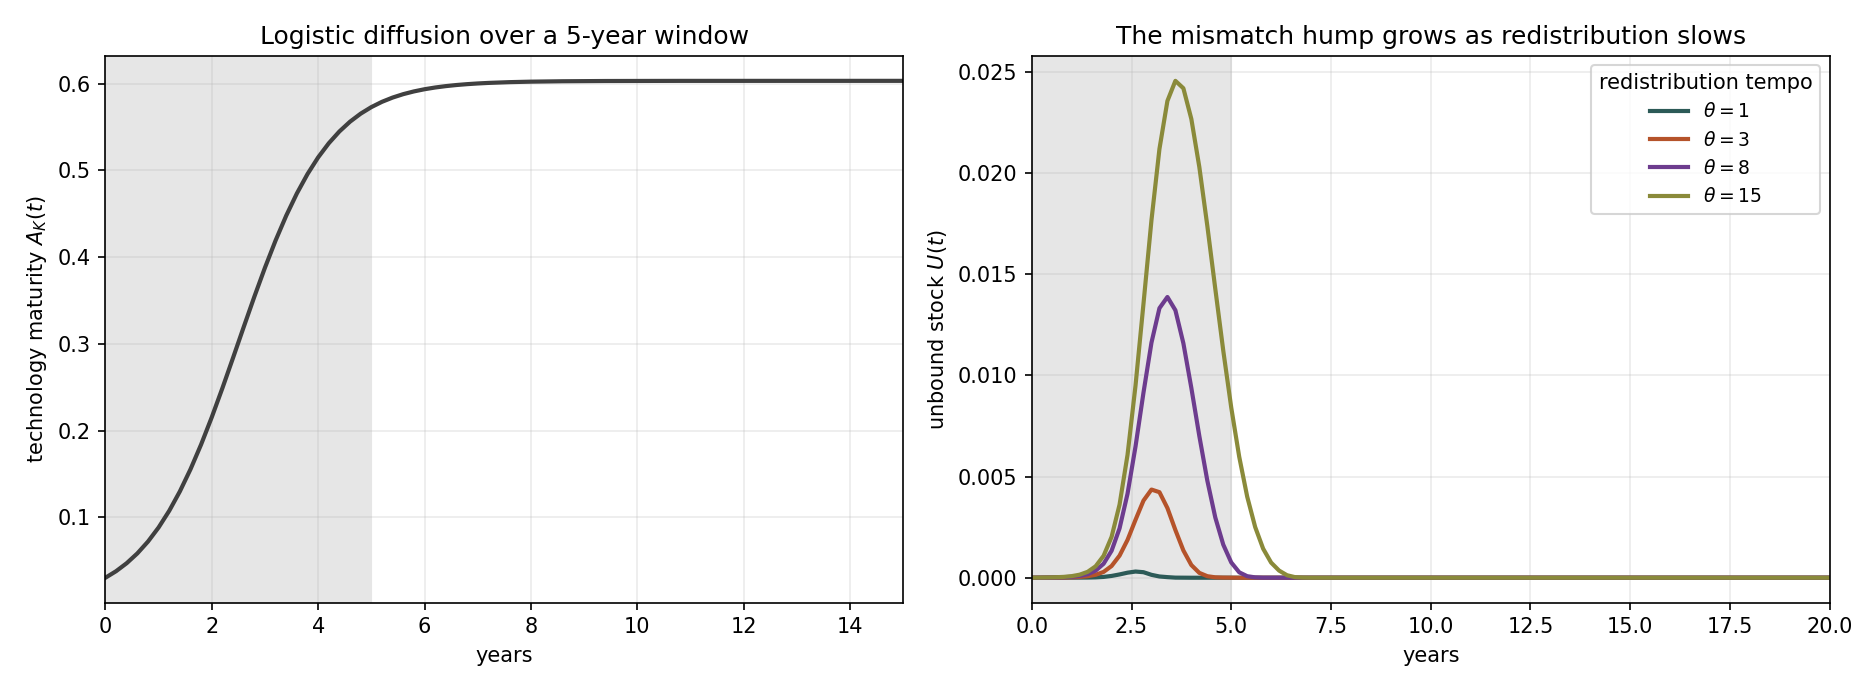
\includegraphics[width=\textwidth]{calendar_dynamics.png}
\caption{Calendar-time dynamics. Left: the technology matures as a
logistic diffusion over a five-year window. Right: the unbound stock
$U(t)$, the transitional mismatch between destruction and creation, for
four redistribution tempos $\theta$ against the fixed five-year shock.
The mismatch hump grows and lingers as redistribution slows relative to
the shock, but always drains to zero: the transitional cost is in the
path, not the endpoint.}
\label{fig:calendar}
\end{figure}

\subsection{The destination depends on the tempo}
\label{sec:destination}

The hump measures the cost of the transition; the same ratio also
determines its outcome. Figure~\ref{fig:tempo} shows where the reinstated
work is bound in two regimes, run through the same technology and the
same field. In the gradual regime, with redistribution faster than the
shock, the best-matched occupations keep pace and absorb the work: the
gainers are the high-skill specialists whose capabilities sit at the
frontier of the field. In the congested regime, with redistribution much
slower than the shock, the small best-matched occupations cannot bind
fast enough --- their size-limited capacity $c_o = M_o/\theta$ is small,
the mass accumulates in $U$, and it is taken instead by the large,
lower-skilled occupations that can absorb it quickly. The same work is
downgraded.

The shift is not marginal. The final allocations of reinstated mass in
the two regimes correlate at roughly $0.3$: substantially different
destinations from one technology and one field, differing only in the
tempo of the shock relative to the market's capacity to respond. This is
the destination counterpart of the transitional hump, and it is a
statement the equilibrium framework cannot make. The fixed point sees the
endpoint of a frictionless reallocation; it cannot see that the endpoint
the economy actually reaches depends on how fast it was forced to move.

\begin{figure}[t]
\centering

\includegraphics[width=\textwidth]{tempo_regimes.png}
\caption{The destination of reinstated work depends on the tempo ratio.
Both panels show the reinstated task mass gained by each occupation, over
the survival-gated seeding field (grey) with the technology field dashed,
for the same five-year shock. Left, a gradual transition: the best
matches keep pace and high-skill specialists at the frontier absorb the
work. Right, a congested transition: small best-matched occupations
cannot keep up and the work is forced onto large, lower-skilled
occupations. The two final allocations correlate at roughly $0.3$.}
\label{fig:tempo}
\end{figure}

\todo{Add the per-occupation evidence behind the figure: the
size-versus-match correlation in each regime, the quartile shares of
absorption, and a short table of the leading gainers in each regime.
Replace any relative-change ranking with absolute and spatial measures,
since the relative measure is unbounded for small occupations.}

\section{The general-equilibrium price feedback}
\label{sec:ge-feedback}

Both the static regime and the dynamic transition above hold the price field
$\Pi(r)$ fixed: the shock relocates labour and re-sorts it, congestion adjusts
the marginal value of crowded destinations, but the per-unit price of capability
content does not re-solve. This is a short-run reading. The price field is an
equilibrium object --- Section~\ref{sec:microfoundation} derives it as a
capability assignment --- and an equilibrium that does not equilibrate discards
its own content. \textcite{acemoglu2024rents} make the point sharply: in their
task model the base wage \emph{adjusts} to automation (their propagation matrix
$\Theta$), and that adjustment is the mechanism. Our fixed-price layers hold even
more fixed than they do --- both the rent wedge and the base price --- so to
``derive the prices'' in their sense we must let the base price move. This
section closes that loop.

\paragraph{The closure: level from data, change from the assignment.}
We keep the level from the estimated field --- the empirical anchor --- and take
the \emph{change} from the assignment, exactly as \textcite{acemoglu2024rents}
take the wage level as given and compute its response. Their wage law
$w_g \propto (\Gamma_g/\ell_g)^{1/\lambda}$ ties the wage to tasks per worker;
its spatial form is
\begin{equation}
  \Delta \ln \Pi(r) \;=\; \frac{1}{\sigma}\Big[\,\ln\big(1-a(r)\big) \;-\; \ln\frac{n_L(r)}{n_L^0(r)}\,\Big],
  \label{eq:price-feedback}
\end{equation}
applied to the baseline, $\Pi(r) = \Pi_0(r)\,e^{\Delta\ln\Pi(r)}$. Automation is a
\emph{demand} shock to labour: where capital takes the task ($a$ high), the task
leaves the human set and the wage falls; and displaced labour crowding the
remaining work ($n_L > n_L^0$) lowers it further. Both terms are stabilising. The
sign is not innocuous: the opposite reading --- treating automation as a
\emph{supply} shock that makes scarce human work dearer --- inverts
equation~\eqref{eq:price-feedback} and is destabilising, since a dearer wage
opens the takeover gate. Run as a single pass at $\sigma = 3$, the scarcity
reading collapses the labour share to $0.33$ (capital chases the work it has just
made dear), while the demand reading lifts it to $0.83$; the fixed-price value
$0.58$ sits between. The headline is not robust to the sign, which therefore must
be chosen on economic grounds. \textcite{acemoglu2024rents} choose ours:
automation dissipates rents and lowers wages, it does not raise them.

\paragraph{The static fixed point.}
Equation~\eqref{eq:price-feedback} is a contraction --- a lower price closes the
takeover gate, which raises the price back --- so iterating price and allocation
to mutual consistency converges (eight damped steps). The self-consistent state
is an interior point, not the one-pass extreme: the labour share settles at
$0.73$ (against $0.58$ at fixed prices), the price level falls $26$ percent, and
displacement is cut by roughly $44$ percent ($D_o$ from $0.28$ to $0.16$). The
wage adjustment absorbs most of the shock: human work becomes about a quarter
cheaper, capital adopts far less, and the labour share stays high --- but the
harm now sits in the wage \emph{level}, not in employment, which is precisely the
rent- and wage-dissipation of \textcite{acemoglu2024rents}.

\paragraph{The dynamic close, and statics meeting dynamics.}
Wired into the transition --- the price responding to the current adoption and
allocation at every step, equation~\eqref{eq:price-feedback} with a one-step lag
--- the feedback shapes the whole path, not just the end. The wage level falls
monotonically as adoption rises, from $-0.09$ early to a plateau at $-0.29$, and
the displacement wave is markedly gentler: the unbound-mass (mismatch) peak is
cut by about $64$ percent (from $0.44$ to $0.16$ percent of the workforce) at the
same timing, and the reinstated stock ends lower, because the falling wage deters
the automation that would have produced the mismatch. Crucially, the transition
lands where the static fixed point says it should: the dynamic end-state price
level ($-0.285$) and labour share ($0.739$) reproduce the static fixed point
($-0.26$, $0.73$) to within rounding. Two independent constructions --- static
fixed-point iteration and dynamic time-stepping --- reach the same equilibrium,
so the price feedback is a property of the model rather than of either method,
and the static and dynamic accounts cohere.

\paragraph{What this does and does not establish.}
The feedback is first-order: at fixed prices both layers overstate the
displacement and understate the labour share, and they overstate the violence of
the transition. The stabilising wage adjustment is the shock absorber, and it
operates throughout the transition, not only at its end. The quantitative point
estimate depends on the assignment elasticity $\sigma$ and on the reduced-form
closure --- equation~\eqref{eq:price-feedback} is the AR wage law applied
region-wise, not a full re-solve of the assignment programme of
Section~\ref{sec:microfoundation} --- and the AI field remains one illustrative
instance of a technology field, not a measurement. We therefore read the result
as establishing the \emph{direction and order of magnitude} of the price
feedback, and the mutual consistency of the static and dynamic closes, rather
than a calibrated forecast of the labour share.

%% ============================================================
\section{Discussion}
\label{sec:discussion}
%% ============================================================

The result is that the tempo of a technology shock, relative to the speed
at which the labour market reallocates, is not merely a determinant of
how painful the transition is but of its outcome. A gradual diffusion
lets work find the occupations whose capabilities match it; a shock that
outruns adjustment forces a downgrading that persists in the final
allocation. The same field, the same displaced mass, and the same seeded
reinstatement yield different societies depending on the pace. This is a
genuinely dynamic statement, and it is the kind of statement the
task-based equilibrium framework is not built to make: its rest point is
the destination of a frictionless economy, and the friction here is time
itself.

Two qualifications bound the claim, and both are inherited rather than
introduced. The first is the survival gate. The companion model places
surviving reinstatement on the low-priced side of the boundary, because a
seeded task is retained by labour where labour is the cheaper producer at
a \emph{uniform} cost $R$, which is the low-$\Pi$, cheaper work. The
reinstated work is therefore lower-priced to begin with, and the
congested regime compounds this by routing it to the large low-skill
occupations. Whether reinstatement \emph{ought} to be lower-skilled is a
question about the survival gate, not the binding law: in
\textcite{acemoglu2019automation} reinstatement is new \emph{complex}
work in which labour has a comparative advantage, often higher-skilled,
and capturing that would require the survival condition to turn on
relative rather than absolute productivity --- a varying human
productivity field, high where the machine is weak, in place of a uniform
$R$. That is a change to the static foundation, deferred here and flagged
in the companion paper. The destination results are therefore conditional
on the survival-gate economics, exactly as the companion paper's
incidence results are. \todo{Decide how far to take the
comparative-advantage qualification here versus leaving it entirely to
the foundation paper. At minimum, state plainly that the high- versus
low-skill character of the gainers is conditional on the gate.}

The second qualification is the binding calibration. The allocation
depends on the sharpness $\beta$ and the absorption timescale
$\theta_{\text{abs}}$, and the central result is presented as a sweep over
the tempo precisely so that the dependence is exhibited rather than
hidden. But the regime boundary --- how slow redistribution must be,
relative to the shock, for downgrading to set in --- is a quantitative
claim that rests on these handles, and a reader is owed their economic
interpretation and the result's sensitivity to them.

Several limitations remain. The realisation is illustrative, inheriting
the companion paper's calibration and its discipline: no causal claim is
made from it. The unbound stock drains to zero, so the model has no
permanent mismatch and no involuntary non-employment; the transitional
cost is the hump, and a model with task decay or irreversible binding
would carry a permanent imprint of the shock speed that this one does
not. New tasks enter as added weight on existing locations rather than as
new points on the disk. And the relative-change measure of who gains is
unbounded for small occupations, so the destination results should be
read in absolute and spatial terms.

\todo{Relate to the adjustment-cost and mismatch literatures once the
framing is fixed; decide whether the permanent-imprint extension (task
decay or forced downgrading that does not reverse) belongs here as a
remark or in a further paper.}

%% ============================================================
\section{Conclusion}
\label{sec:conclusion}
%% ============================================================

Turning the spatial task-based model from an equilibrium into laws of
motion requires one new object, a stock of unbound task mass, and yields
two things the equilibrium cannot. The first is the transitional
mismatch $U(t)$, the gap between destruction and creation as a transient
that grows with the tempo of the shock and drains as the market catches
up. The second, and the central result, is that the tempo of the shock
relative to the speed of redistribution determines the destination of the
reinstated work: a gradual shock matches it to high-skill specialists, a
fast shock forces it onto large lower-skilled occupations. The same
technology yields a different distribution of work depending only on how
fast it arrives. The cost and the outcome of automation are, in this
sense, properties of the path and not only of the endpoint.

%% ============================================================
\printbibliography
%% ============================================================

\todo{Bibliography keys to add/verify in references.bib:
storck2026fields (the companion static paper, ``Technology fields,
automation and task reinstatement'', Storck \& Andersson, 2026 --- the
foundation cited throughout); storck2026geometry (Paper 1, polar
geometry, already in references.bib); acemoglu2018race,
acemoglu2019automation, bessen2019demand (already needed by the companion
paper). No new external references are strictly required for this draft;
all machinery is inherited. Verify each against full text before
submission.}

\end{document}